% Options for packages loaded elsewhere
\PassOptionsToPackage{unicode}{hyperref}
\PassOptionsToPackage{hyphens}{url}
\PassOptionsToPackage{dvipsnames,svgnames,x11names}{xcolor}
%
\documentclass[
  letterpaper,
  DIV=11,
  numbers=noendperiod]{scrartcl}

\usepackage{amsmath,amssymb}
\usepackage{iftex}
\ifPDFTeX
  \usepackage[T1]{fontenc}
  \usepackage[utf8]{inputenc}
  \usepackage{textcomp} % provide euro and other symbols
\else % if luatex or xetex
  \usepackage{unicode-math}
  \defaultfontfeatures{Scale=MatchLowercase}
  \defaultfontfeatures[\rmfamily]{Ligatures=TeX,Scale=1}
\fi
\usepackage{lmodern}
\ifPDFTeX\else  
    % xetex/luatex font selection
  \setmainfont[]{Inter}
  \setsansfont[]{Inter}
  \setmathfont[]{Fira Math}
\fi
% Use upquote if available, for straight quotes in verbatim environments
\IfFileExists{upquote.sty}{\usepackage{upquote}}{}
\IfFileExists{microtype.sty}{% use microtype if available
  \usepackage[]{microtype}
  \UseMicrotypeSet[protrusion]{basicmath} % disable protrusion for tt fonts
}{}
\makeatletter
\@ifundefined{KOMAClassName}{% if non-KOMA class
  \IfFileExists{parskip.sty}{%
    \usepackage{parskip}
  }{% else
    \setlength{\parindent}{0pt}
    \setlength{\parskip}{6pt plus 2pt minus 1pt}}
}{% if KOMA class
  \KOMAoptions{parskip=half}}
\makeatother
\usepackage{xcolor}
\setlength{\emergencystretch}{3em} % prevent overfull lines
\setcounter{secnumdepth}{5}
% Make \paragraph and \subparagraph free-standing
\ifx\paragraph\undefined\else
  \let\oldparagraph\paragraph
  \renewcommand{\paragraph}[1]{\oldparagraph{#1}\mbox{}}
\fi
\ifx\subparagraph\undefined\else
  \let\oldsubparagraph\subparagraph
  \renewcommand{\subparagraph}[1]{\oldsubparagraph{#1}\mbox{}}
\fi


\providecommand{\tightlist}{%
  \setlength{\itemsep}{0pt}\setlength{\parskip}{0pt}}\usepackage{longtable,booktabs,array}
\usepackage{calc} % for calculating minipage widths
% Correct order of tables after \paragraph or \subparagraph
\usepackage{etoolbox}
\makeatletter
\patchcmd\longtable{\par}{\if@noskipsec\mbox{}\fi\par}{}{}
\makeatother
% Allow footnotes in longtable head/foot
\IfFileExists{footnotehyper.sty}{\usepackage{footnotehyper}}{\usepackage{footnote}}
\makesavenoteenv{longtable}
\usepackage{graphicx}
\makeatletter
\def\maxwidth{\ifdim\Gin@nat@width>\linewidth\linewidth\else\Gin@nat@width\fi}
\def\maxheight{\ifdim\Gin@nat@height>\textheight\textheight\else\Gin@nat@height\fi}
\makeatother
% Scale images if necessary, so that they will not overflow the page
% margins by default, and it is still possible to overwrite the defaults
% using explicit options in \includegraphics[width, height, ...]{}
\setkeys{Gin}{width=\maxwidth,height=\maxheight,keepaspectratio}
% Set default figure placement to htbp
\makeatletter
\def\fps@figure{htbp}
\makeatother

\usepackage{amsmath, xparse}
\usepackage{fancyvrb, fvextra}
\usepackage{unicode-math}
\usepackage{svg}
\usepackage{multicol}
\usepackage{listings}
\usepackage{systeme}
\usepackage{xifthen}
\DefineVerbatimEnvironment{Highlighting}{Verbatim}{breaklines,commandchars=\\\{\}}
\lstset{basicstyle=\ttfamily\footnotesize,breaklines=true}
\newcommand\rowop[1]{\scriptstyle\smash{\xrightarrow[\vphantom{#1}]{\mkern-4mu#1\mkern-4mu}}}
\DeclareDocumentCommand\converttorows%
{>{\SplitList{,}}m}%
{\ProcessList{#1}{\converttorow}}
\NewDocumentCommand{\converttorow}{m}
{\ifthenelse{\isempty{#1}}{}{\rowop{#1}}\\}

\DeclareDocumentCommand \rowops{m}
{\;
\begin{matrix}
\converttorows {#1}
\end{matrix}
\; }
\KOMAoption{captions}{tableheading}
\makeatletter
\makeatother
\makeatletter
\makeatother
\makeatletter
\@ifpackageloaded{caption}{}{\usepackage{caption}}
\AtBeginDocument{%
\ifdefined\contentsname
  \renewcommand*\contentsname{Table of contents}
\else
  \newcommand\contentsname{Table of contents}
\fi
\ifdefined\listfigurename
  \renewcommand*\listfigurename{List of Figures}
\else
  \newcommand\listfigurename{List of Figures}
\fi
\ifdefined\listtablename
  \renewcommand*\listtablename{List of Tables}
\else
  \newcommand\listtablename{List of Tables}
\fi
\ifdefined\figurename
  \renewcommand*\figurename{Figure}
\else
  \newcommand\figurename{Figure}
\fi
\ifdefined\tablename
  \renewcommand*\tablename{Table}
\else
  \newcommand\tablename{Table}
\fi
}
\@ifpackageloaded{float}{}{\usepackage{float}}
\floatstyle{ruled}
\@ifundefined{c@chapter}{\newfloat{codelisting}{h}{lop}}{\newfloat{codelisting}{h}{lop}[chapter]}
\floatname{codelisting}{Listing}
\newcommand*\listoflistings{\listof{codelisting}{List of Listings}}
\makeatother
\makeatletter
\@ifpackageloaded{caption}{}{\usepackage{caption}}
\@ifpackageloaded{subcaption}{}{\usepackage{subcaption}}
\makeatother
\makeatletter
\@ifpackageloaded{tcolorbox}{}{\usepackage[skins,breakable]{tcolorbox}}
\makeatother
\makeatletter
\@ifundefined{shadecolor}{\definecolor{shadecolor}{rgb}{.97, .97, .97}}
\makeatother
\makeatletter
\makeatother
\makeatletter
\makeatother
\ifLuaTeX
  \usepackage{selnolig}  % disable illegal ligatures
\fi
\IfFileExists{bookmark.sty}{\usepackage{bookmark}}{\usepackage{hyperref}}
\IfFileExists{xurl.sty}{\usepackage{xurl}}{} % add URL line breaks if available
\urlstyle{same} % disable monospaced font for URLs
\hypersetup{
  colorlinks=true,
  linkcolor={blue},
  filecolor={Maroon},
  citecolor={Blue},
  urlcolor={Blue},
  pdfcreator={LaTeX via pandoc}}

\author{}
\date{}

\begin{document}
\begin{titlepage}

    \newcommand{\HRule}{\rule{\linewidth}{0.5mm}}
    
    \center
    
    \vspace{10cm}

    \textsc{\LARGE Gwinnett School of Math, Science, and Technology }\\[0.3cm]
    
    \vspace{0.5cm}

    \HRule \\[0.4cm]
    { \huge \bfseries Macroeconomics Yearlong Notes}\\[0.03cm]
    \HRule \\[1.5cm]
    
    \begin{minipage}{0.4\textwidth}
    \begin{flushleft} \Large
    Anish Goyal \\1st Period
    \end{flushleft}
    \end{minipage}
    ~
    \begin{minipage}{0.4\textwidth}
    \begin{flushright} \Large
    Michael Burbine\\Educator
    \end{flushright}
    \end{minipage}\\[1cm]
    
    {\huge 2023-2024}\\[1cm]
    
    
\includegraphics{img/logo.png}\\
    \vfill
    \end{titlepage}

\newpage

\ifdefined\Shaded\renewenvironment{Shaded}{\begin{tcolorbox}[interior hidden, boxrule=0pt, sharp corners, frame hidden, borderline west={3pt}{0pt}{shadecolor}, enhanced, breakable]}{\end{tcolorbox}}\fi

\renewcommand*\contentsname{Table of Contents}
{
\hypersetup{linkcolor=}
\setcounter{tocdepth}{4}
\tableofcontents
}
\newpage{}

\hypertarget{types-of-goods-0108}{%
\section{Types of Goods (01/08)}\label{types-of-goods-0108}}

\hypertarget{characteristics-of-the-four-types-of-goods}{%
\subsection{Characteristics of the Four Types of
Goods}\label{characteristics-of-the-four-types-of-goods}}

\begin{itemize}
\tightlist
\item
  \textbf{Rivalrous} goods are those that can only be consumed by one
  person at a time.
\item
  \textbf{Non-rivalrous} goods are those that can be consumed by
  multiple people at the same time.
\item
  \textbf{Excludable} goods are those that can be restricted to certain
  people.
\item
  \textbf{Non-excludable} goods are those that cannot be restricted to
  certain people.
\item
  If a public good is overcrowded enough, it can become a common
  resource
\end{itemize}

\hypertarget{the-four-types-of-goods}{%
\subsection{The Four Types of Goods}\label{the-four-types-of-goods}}

\begin{longtable}[]{@{}
  >{\raggedright\arraybackslash}p{(\columnwidth - 4\tabcolsep) * \real{0.1667}}
  >{\raggedright\arraybackslash}p{(\columnwidth - 4\tabcolsep) * \real{0.4762}}
  >{\raggedright\arraybackslash}p{(\columnwidth - 4\tabcolsep) * \real{0.3492}}@{}}
\toprule\noalign{}
\begin{minipage}[b]{\linewidth}\raggedright
\end{minipage} & \begin{minipage}[b]{\linewidth}\raggedright
\textbf{Non-rivalrous}
\end{minipage} & \begin{minipage}[b]{\linewidth}\raggedright
\textbf{Rivalrous}
\end{minipage} \\
\midrule\noalign{}
\endhead
\bottomrule\noalign{}
\endlastfoot
\textbf{Non-excludable} & \begin{minipage}[t]{\linewidth}\raggedright
\emph{Public Goods}\\
(e.g.~Sunset, Common Knowledge)\strut
\end{minipage} & \begin{minipage}[t]{\linewidth}\raggedright
\emph{Common-Pool/Common Resources}\\
(e.g.~Irrigation Systems, Libraries)\strut
\end{minipage} \\
\textbf{Excludable} & \begin{minipage}[t]{\linewidth}\raggedright
\emph{(Toll/Club/Artificially Scarce) Goods/Natural monopolies}\\
(e.g.~Day-Care Centers, Country Clubs)\strut
\end{minipage} & \begin{minipage}[t]{\linewidth}\raggedright
\emph{Private Goods}\\
(e.g.~Donuts, Personal Computers)\strut
\end{minipage} \\
\end{longtable}

\hypertarget{examples}{%
\subsection{Examples}\label{examples}}

\begin{longtable}[]{@{}
  >{\raggedright\arraybackslash}p{(\columnwidth - 2\tabcolsep) * \real{0.7042}}
  >{\raggedright\arraybackslash}p{(\columnwidth - 2\tabcolsep) * \real{0.2958}}@{}}
\toprule\noalign{}
\begin{minipage}[b]{\linewidth}\raggedright
Case Scenario
\end{minipage} & \begin{minipage}[b]{\linewidth}\raggedright
Type of Good/Service
\end{minipage} \\
\midrule\noalign{}
\endhead
\bottomrule\noalign{}
\endlastfoot
A college education & Artificially scarce \\
A manicure or pedicure & Private good \\
Stone Mountain park & Artificially scarce \\
State park campgrounds & Artificially scarce \\
National defense & Public good \\
Peach Pass lane on I-85 & Artificially scarce \\
Fish in the ocean & Common resource \\
Street lights & Public good \\
Netflix/Hulu & Artificially scarce \\
Flu shot & Private good \\
Tornado safety shelter & Public good \\
Bottled water in a tornado safety shelter & Common resource \\
Hearing a tornado siren & Public good \\
Going to an almost empty public beach & Public good \\
Going to an overcrowded public beach & Common resource \\
St.~Lawrence SeaWay & Natural monopoly \\
Flying on a commercial airplane & Natural monopoly \\
Flying a single seat private airplane & Private good \\
Wedding guests eating a slice of the wedding-cake & Common resource \\
Cake sold at a bakery & Private good \\
\end{longtable}

\hypertarget{introduction-to-externalities-0109}{%
\section{Introduction to Externalities
(01/09)}\label{introduction-to-externalities-0109}}

\begin{itemize}
\tightlist
\item
  An \textbf{externality} is a cost/benefit that affects a \emph{third
  party} who did not choose to incur that cost/benefit.
\item
  They are a type of \textbf{market failure} because they are \emph{not}
  accounted for in the price of the good/service.
\item
  The DWL of positive externalities will point to the right and
  vice-versa for negative externalities.

  \begin{itemize}
  \tightlist
  \item
    It also always points to the social optimum quantity.
  \end{itemize}
\end{itemize}

\hypertarget{positive-externality-in-consumption}{%
\subsection{Positive Externality in
Consumption}\label{positive-externality-in-consumption}}

\begin{figure}

{\centering 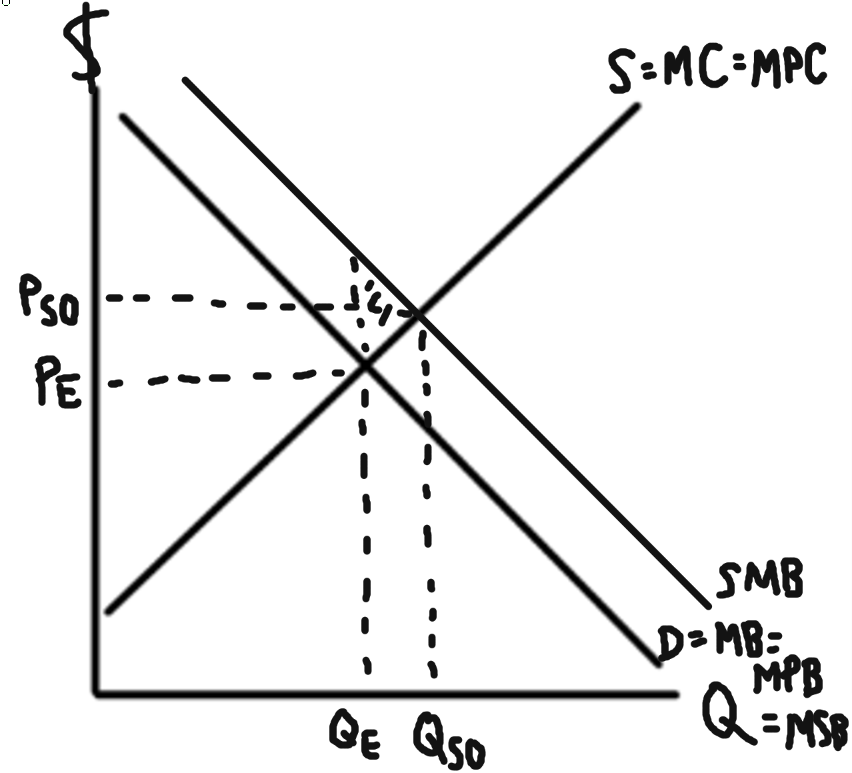
\includegraphics[width=0.5\textwidth,height=\textheight]{img/pos-cons.png}

}

\caption{Positive Externality in Consumption}

\end{figure}

\hypertarget{examples-1}{%
\subsubsection{Examples}\label{examples-1}}

\begin{itemize}
\tightlist
\item
  Consumption of education
\item
  Consumption of health care
\item
  Advertisement can lead to an increase of demand in the free market
  \(\therefore MPB\) goes up and moves the market toward \(MSB\).
\end{itemize}

\hypertarget{spillover-effect}{%
\subsubsection{Spillover Effect}\label{spillover-effect}}

\begin{itemize}
\tightlist
\item
  The spillover effect is \(MSB = MPB+MEB\).
\item
  \(MPB = MSB\)
\item
  \(MB > MSB\)
\end{itemize}

\hypertarget{internalizing-the-spillover-effect}{%
\subsubsection{Internalizing the Spillover
Effect}\label{internalizing-the-spillover-effect}}

The external \textbf{benefits} can be internalized by
\textbf{subsidizing} the product/service to the consumers of the
good/service.

\newpage{}

\hypertarget{negative-externality-in-consumption}{%
\subsection{Negative Externality in
Consumption}\label{negative-externality-in-consumption}}

\begin{figure}

{\centering 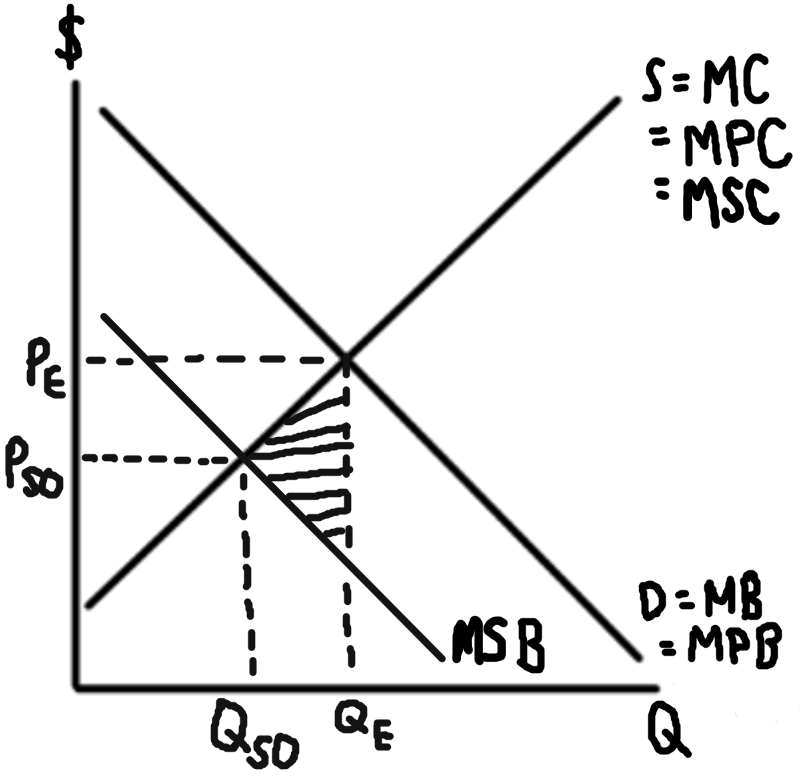
\includegraphics[width=0.5\textwidth,height=\textheight]{img/neg-cons.png}

}

\caption{Negative Externality in Consumption}

\end{figure}

\hypertarget{examples-2}{%
\subsubsection{Examples}\label{examples-2}}

\begin{itemize}
\tightlist
\item
  Smoking in public/passive smoking
\item
  Pollution due to fossil fuels
\item
  Playing loud music
\item
  Discarding garbage in public places
\end{itemize}

\hypertarget{spillover-effect-1}{%
\subsubsection{Spillover Effect}\label{spillover-effect-1}}

\begin{itemize}
\tightlist
\item
  The spillover effect is \(MSB = MPB-MEB\).
\item
  \(MPB = MSB\)
\item
  \(MB < MSB\)
\end{itemize}

\hypertarget{internalizing-the-spillover-effect-1}{%
\subsubsection{Internalizing the Spillover
Effect}\label{internalizing-the-spillover-effect-1}}

The external \textbf{costs} can be internalized by \textbf{imposing a
tax} on the product/service to the consumers of the good/service.

\newpage{}

\hypertarget{positive-externality-in-production}{%
\subsection{Positive Externality in
Production}\label{positive-externality-in-production}}

\begin{figure}

{\centering 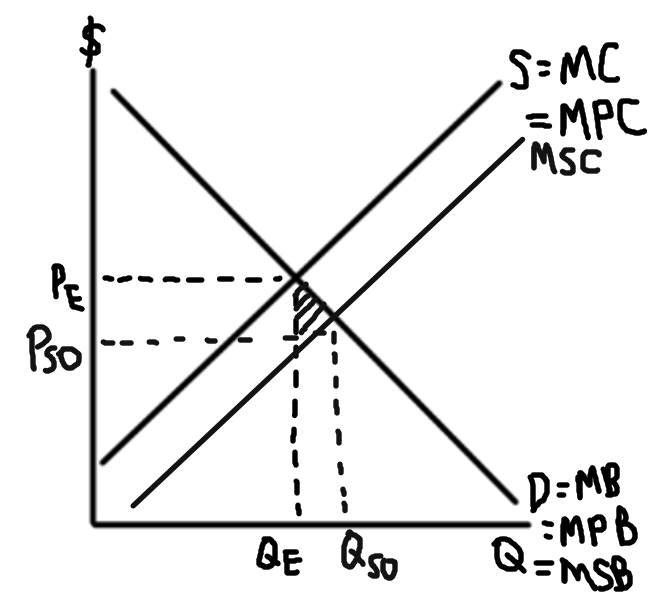
\includegraphics[width=0.5\textwidth,height=\textheight]{img/pos-prod.png}

}

\caption{Positive Externality in Production}

\end{figure}

\hypertarget{examples-3}{%
\subsubsection{Examples}\label{examples-3}}

\begin{itemize}
\tightlist
\item
  Companies invest in training/professional development of their
  employees.
\item
  Firms invest in research and development (R\&D).
\end{itemize}

\hypertarget{spillover-effect-2}{%
\subsubsection{Spillover Effect}\label{spillover-effect-2}}

\begin{itemize}
\tightlist
\item
  The spillover effect is \(MSC = MPC-MEC\).
\item
  \(MPB = MSC\)
\item
  \(MC > MSC\)
\end{itemize}

\hypertarget{internalizing-the-spillover-effect-2}{%
\subsubsection{Internalizing the Spillover
Effect}\label{internalizing-the-spillover-effect-2}}

The external \textbf{benefits} can be internalized by
\textbf{subsidizing} the product/service to the producers of the
good/service.

\newpage{}

\hypertarget{negative-externality-in-production}{%
\subsection{Negative Externality in
Production}\label{negative-externality-in-production}}

\begin{figure}

{\centering 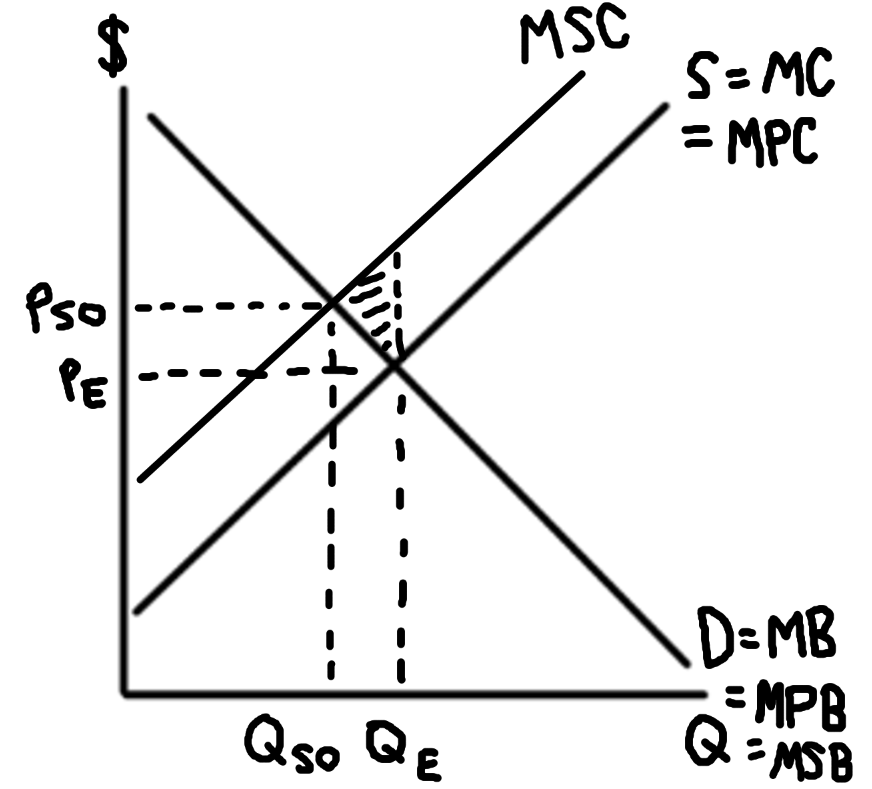
\includegraphics[width=0.5\textwidth,height=\textheight]{img/neg-prod.png}

}

\caption{Negative Externality in Production}

\end{figure}

\hypertarget{examples-4}{%
\subsubsection{Examples}\label{examples-4}}

\begin{itemize}
\tightlist
\item
  Firms produce chemicals that cause pollution \(therefore\) local
  fisherman cannot catch fish.
\item
  Construction of roads lead to change of landscape and parks
\item
  Coal fired power plants
\end{itemize}

\hypertarget{spillover-effect-3}{%
\subsubsection{Spillover Effect}\label{spillover-effect-3}}

\begin{itemize}
\tightlist
\item
  The spillover effect is \(MSC = MPC+MEC\).
\item
  \(MPB = MSC\)
\item
  \(MC < MSC\)
\end{itemize}

\hypertarget{internalizing-the-spillover-effect-3}{%
\subsubsection{Internalizing the Spillover
Effect}\label{internalizing-the-spillover-effect-3}}

\begin{itemize}
\tightlist
\item
  The external \textbf{costs} can be internalized by \textbf{imposing a
  tax} on the product/service to the producers of the good/service.
\item
  The government intervention will move the private market to
  \textbf{social optimum} where \(MSB = MSC\).
\end{itemize}

\newpage{}



\end{document}
